\newpage
\stepcounter{handout}

%%% FSM

\begin{exercisebox}[adjusted title= Finite state machines - Traffic Light]
\textbf{Look in the samples folder for the script}
\mbox{\url{https://editor.p5js.org/spikol/sketches/wM_mzde00}}

\begin{lstlisting}[language=JavaScript]
// States for our FSM (Finite State Machine)
const STATE_RED = "RED";
const STATE_GREEN = "GREEN";


// Initial state
let current_state = STATE_RED;

function setup() {
 // Create a canvas with a width and height of 200 pixels
  createCanvas(200, 200); 
  fill(255);  // Set the default fill color to white
}

function draw() {
  background(200);  // Set the background color to a light gray
  
  // Check the current state and set the fill color accordingly
  if (current_state === STATE_RED) {
    fill(255, 0, 0);  // Red color for RED state
  } else if (current_state === STATE_GREEN) {
    fill(0, 255, 0);  // Green color for GREEN state
  } 
  // Draw a circle in the center of the canvas
  ellipse(width / 2, height / 2, 100, 100);  
}

function mousePressed() {
  // Update the state based on the current state
  if (current_state === STATE_RED) {
    current_state = STATE_GREEN;
  } else if (current_state === STATE_GREEN) {
    current_state = STATE_RED;
  } 
}
\end{lstlisting}
\end{exercisebox}

\begin{exercisebox}[adjusted title= Details- Traffic Light]
\begin{enumerate}
    \item \textbf{State Constants:}
    \begin{itemize}
        \item The state variables \texttt{STATE\_RED}, \texttt{STATE\_GREEN} are directly converted to JavaScript constants using \texttt{const}.
    \end{itemize}

    \item \textbf{Initial State:}
    \begin{itemize}
        \item The initial state is set using \texttt{let current\_state = STATE\_RED;} to indicate the starting state.
    \end{itemize}

    \item \textbf{setup() Function:}
    \begin{itemize}
        \item \texttt{createCanvas(200, 200)} is used to set up a 200x200 pixel canvas.
        \item \texttt{fill(255)} sets the initial fill color to white, though this will be overridden in \texttt{draw()} based on the state.
    \end{itemize}

    \item \textbf{draw() Function:}
    \begin{itemize}
        \item The \texttt{draw()} function is called repeatedly to render the scene.
        \item It checks the current state (\texttt{current\_state}) and sets the fill color accordingly (red or greeen).
        \item A circle is drawn in the center of the canvas using the \texttt{ellipse()} function.
    \end{itemize}

    \item \textbf{mousePressed() Function:}
    \begin{itemize}
        \item The \texttt{mousePressed()} function handles the state transitions when the mouse is pressed.
        \item It cycles through the states (\texttt{STATE\_RED} and \texttt{STATE\_GREEN} in the order specified.
    \end{itemize}
\end{enumerate}
\end{exercisebox}

\begin{exercisebox}[adjusted title= Finite state machines - Task]
\textbf{Your mission is as follows: the traffic light self-destruct.}
\begin{itemize}
\item Add \texttt{STATE\_YELLOW}
\item Remember to add to \texttt{const}
\item Also you will need to modify the \texttt{function draw()} and \texttt{function mousePressed()} for state and the trigger.
\end{itemize}
\end{exercisebox}

\begin{exercisebox}[adjusted title= Finite state machines - Padlock]

\begin{minipage}{1.0\linewidth}
\begin{wrapfigure}[9]{r}{0.15\textwidth}
   \vspace{-1em}
   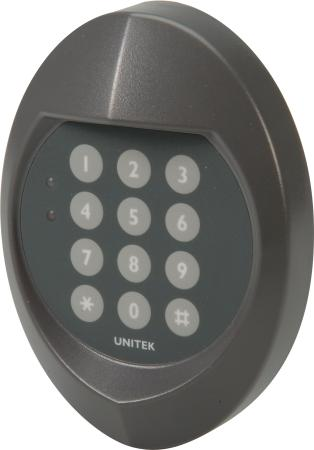
\includegraphics[width=0.15\textwidth]{illustrationer/unitek_kombinationslaas.jpg}
\end{wrapfigure}
 
As the first example of a state machine, we will create one
electronic combination lock, such as those used for access control
doors.

\noindent
Tilstandsdiagram:

\noindent
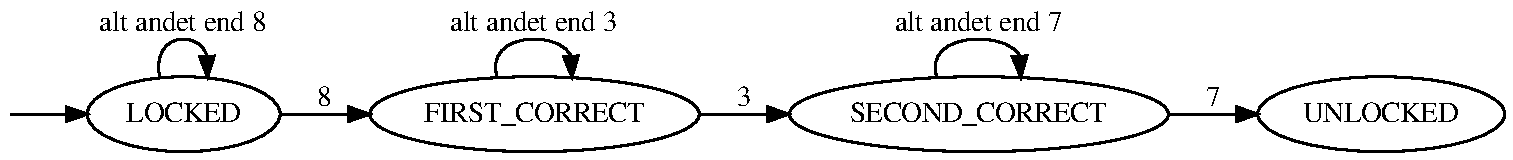
\includegraphics[width=0.85\textwidth]{graphviz/combinationLock_dumb}

%%% FIX!!!!
Copy the p5js code for the combination from the shared collection: 
\mbox{\url{https://editor.p5js.org/spikol/sketches/qqyKLj46m}}

\end{minipage}

\begin{itemize}
\item Test the combination lock and watch as the state changes. If you
did not know the ransom (password), how many attempts does it require?
to guess?

\item Change the code so that the default is 524 instead
\item Try changing the code to follow this diagram instead, where incorrect presses reset the state to start:
 
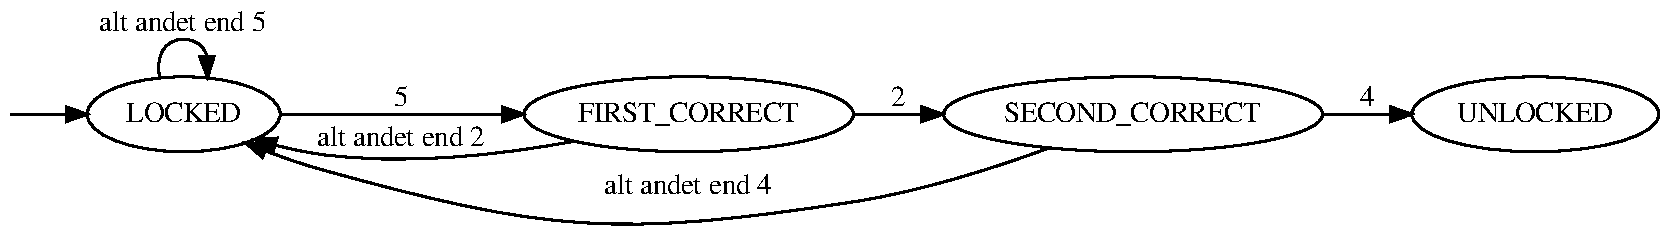
\includegraphics[width=0.85\textwidth]{graphviz/combinationLock_resetting}

\item Draw an extended state diagram of the combination lock with an extra mode, so 4 digits are required. Next, add the extra state in the code.
\end{itemize}
\end{exercisebox}

\begin{exercisebox}[adjusted title= Automatic relock after 2 seconds]

Let's extend the lock so that the door automatically locks again after 2 seconds,
which corresponds to 120 frames:

\noindent
\begin{center}
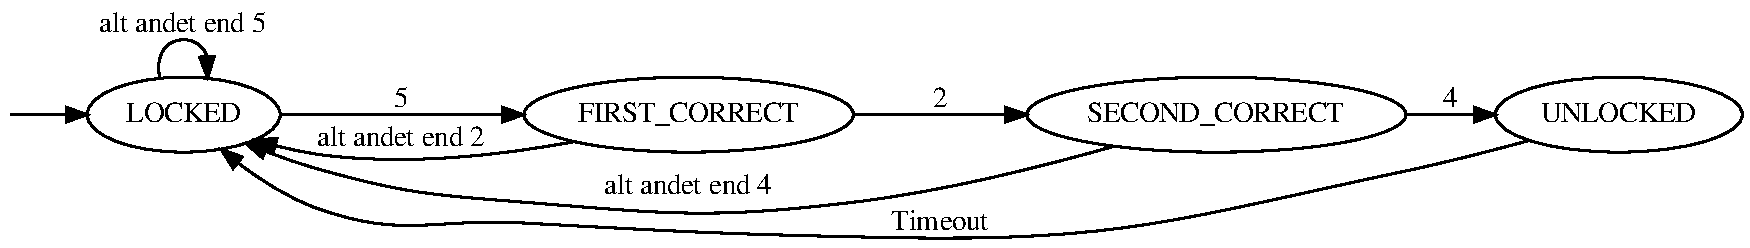
\includegraphics[width=1.0\textwidth]{graphviz/combinationLock_timeout}
\end{center}

\begin{itemize}
\item Create a global variable ``\ttpy{timer}'' and set it to 0
\item Set the \ttpy{timer} variable to 120 as soon as the lock is unlocked. It will
 say when it changes \ttpy{lockState} to \ttpy{"UNLOCKED"}.
\item Count down with the timer in each frame (add the following to the \ttpy{draw} function):

\begin{lstlisting}[language=JavaScript]
if (lockState === "UNLOCKED") {
    drawLock(width / 2, height / 2, 50, true);
    timer -= 1;  // Decrement the timer
\end{lstlisting}

\item The lock must be opened When the timer has counted down. The \ttpy{draw} function must now check if we are in the mode \ttpy{"UNLOCKED"} and the timer simultaneously has counted down to 0. 
\item Paste the following in \ttpy{draw}:
 
\begin{lstlisting}[language=JavaScript]
if (timer === 0) {
    lockState = "LOCKED";  // Reset to LOCKED state when timer runs out
  }
\end{lstlisting}

\end{itemize}
\end{exercisebox}
